\chapter{Generación de código}
\label{cap:generacion-codigo}
\begingroup
\setlength{\emergencystretch}{4em}

La generación de código es la etapa final del compilador TinyS. Recibe el
árbol sintáctico abstracto (AST) construido y validado en las etapas
anteriores, consulta la tabla de símbolos y produce un programa en
ensamblador MIPS. El código resultante incluye la inicialización del
programa, las rutinas de ejecución, las funciones de usuario y el bloque
de entrada \texttt{start}.

\section{Diseño y ejecución de la etapa}
\label{sec:diseno-generacion}

La generación se apoya en el AST y en la tabla de símbolos creados durante
el análisis semántico. El recorrido no vuelve a comprobar los tipos ni la
validez de las declaraciones: utiliza los enlaces ya establecidos por el
analizador para ubicar variables, parámetros, atributos, métodos y clases.

\begin{description}[style=nextline]
  \item[Orquestación]
  \lexcode{TinyS.main()} delega el proceso en
  \lexcode{SemanticStageRunner} con la etapa \texttt{COMPILER}. El
  ejecutador efectúa primero el análisis de declaraciones y luego vuelve
  a leer el fuente para analizar sentencias y construir el AST.
  \item[Inicio del recorrido]
  \lexcode{AST.generate()} inicia la generación sobre el árbol completo.
  Los nodos implementan \lexcode{accept(Visitor<T>)} y delegan la
  operación en la sobrecarga correspondiente del visitante.
  \item[Traducción]
  \lexcode{CodeGenVisitor} implementa \lexcode{Visitor<Void>}. Sus
  métodos \lexcode{visit(...)} emiten las instrucciones de cada expresión
  y sentencia a través de \lexcode{CodeGenerator}.
  \item[Acumulación y salida]
  \lexcode{CodeGenerator} mantiene por separado los datos, las virtual tables, el texto de métodos y el texto de \texttt{start}.
  \lexcode{generate()} concatena esos bloques y
  \lexcode{writeOutput()} escribe el resultado cuando se utiliza desde
  las pruebas de generación.
\end{description}

La compilación completa se ejecuta desde la raíz del proyecto:
\begin{verbatim}
mvn package
java -jar target/tinyS.jar <ARCHIVO_FUENTE>.s
\end{verbatim}
En una compilación satisfactoria, el ejecutador informa
\texttt{CORRECTO: GENERACION DE CODIGO} y escribe junto al fuente los
archivos \texttt{.ts.json}, \texttt{.ast.json} y \texttt{.asm}. La etapa
se ejecuta solo si finalizaron correctamente el análisis léxico,
sintáctico y semántico.

\section{Arquitectura del generador}
\label{sec:arquitectura-generador}

\subsection{Visitante del AST}
\lexcode{CodeGenVisitor} es responsable de traducir los nodos. Las
expresiones dejan su resultado en \texttt{\$a0}, las operaciones que
necesitan preservar valores intermedios los guardan temporalmente en la
pila o en registros temporales (siempre y cuando no se salga del ámbito). Las sentencias emiten instrucciones de
control, asignaciones, llamadas y retornos. El visitante delega en el
generador las operaciones repetidas, como emitir etiquetas, reservar
espacio, acceder a variables y construir prólogos y epílogos.

El visitante separa la traducción en categorías que reflejan el AST:
expresiones, accesos y llamadas, sentencias y bloques. Por ejemplo, una
expresión binaria visita primero el operando izquierdo y preserva su
resultado; luego visita el derecho, recupera ambos valores y emite la
operación correspondiente. Los nodos de control generan etiquetas y
saltos para representar las ramas y los ciclos.

\subsection{Emisor y plantillas}
\lexcode{CodeGenerator} ofrece operaciones para emitir instrucciones,
etiquetas, comentarios y separadores, además de utilidades para manejar
la pila y calcular desplazamientos. Al construirse, carga los recursos
\lexcode{codeGen/data.asm} y \lexcode{codeGen/text.asm}. El primero
contiene datos y tablas de las clases predefinidas, el segundo aporta
rutinas de entrada, salida, arreglos y manejo de errores de ejecución.

El código específico del programa se acumula en cuatro bloques:
\begin{description}[style=nextline]
  \item[Cadenas]
  Literales y etiquetas para datos de tipo cadena.
  \item[Virtual tables]
  Etiquetas y palabras que referencian los métodos asociados a cada clase.
  \item[Texto de métodos]
  Instrucciones de constructores y métodos del programa.
  \item[Texto principal]
  Instrucciones del bloque \texttt{start}, emitidas bajo la etiqueta
  global \texttt{main}.
\end{description}

\lexcode{CodeGenerator.generate()} construye el archivo en este orden:
segmento \texttt{.data}, datos predefinidos, datos de cadenas,
tablas virtuales, segmento \texttt{.text}, símbolo global \texttt{main},
código de \texttt{start}, rutinas de ejecución y métodos generados.

\section{Representación de valores y memoria}
\label{sec:representacion-memoria}

\subsection{Valores primitivos}
Se decidió que todos los valores primitivos se manipulen mediante una referencia a un CIR 
de dos palabras, reservado en el heap. La primera palabra contiene la referencia a la tabla virtual del
tipo cuando corresponde, y la segunda contiene el valor o la dirección del
contenido. Por eso, una expresión primitiva produce en
\texttt{\$a0} la dirección de su CIR, y las operaciones aritméticas,
relacionales o lógicas cargan el contenido antes de operar.

Los CIR de \texttt{Int} y \texttt{Bool} tienen cero en la primera palabra
y almacenan el valor en la segunda. El CIR de \texttt{Str} apunta a
\texttt{vtable\_str} y su segunda palabra apunta a los bytes de la
cadena. La creación de literales y los valores de retorno de las rutinas
predefinidas siguen estas convenciones.

\begin{figure}[H]
  \centering
  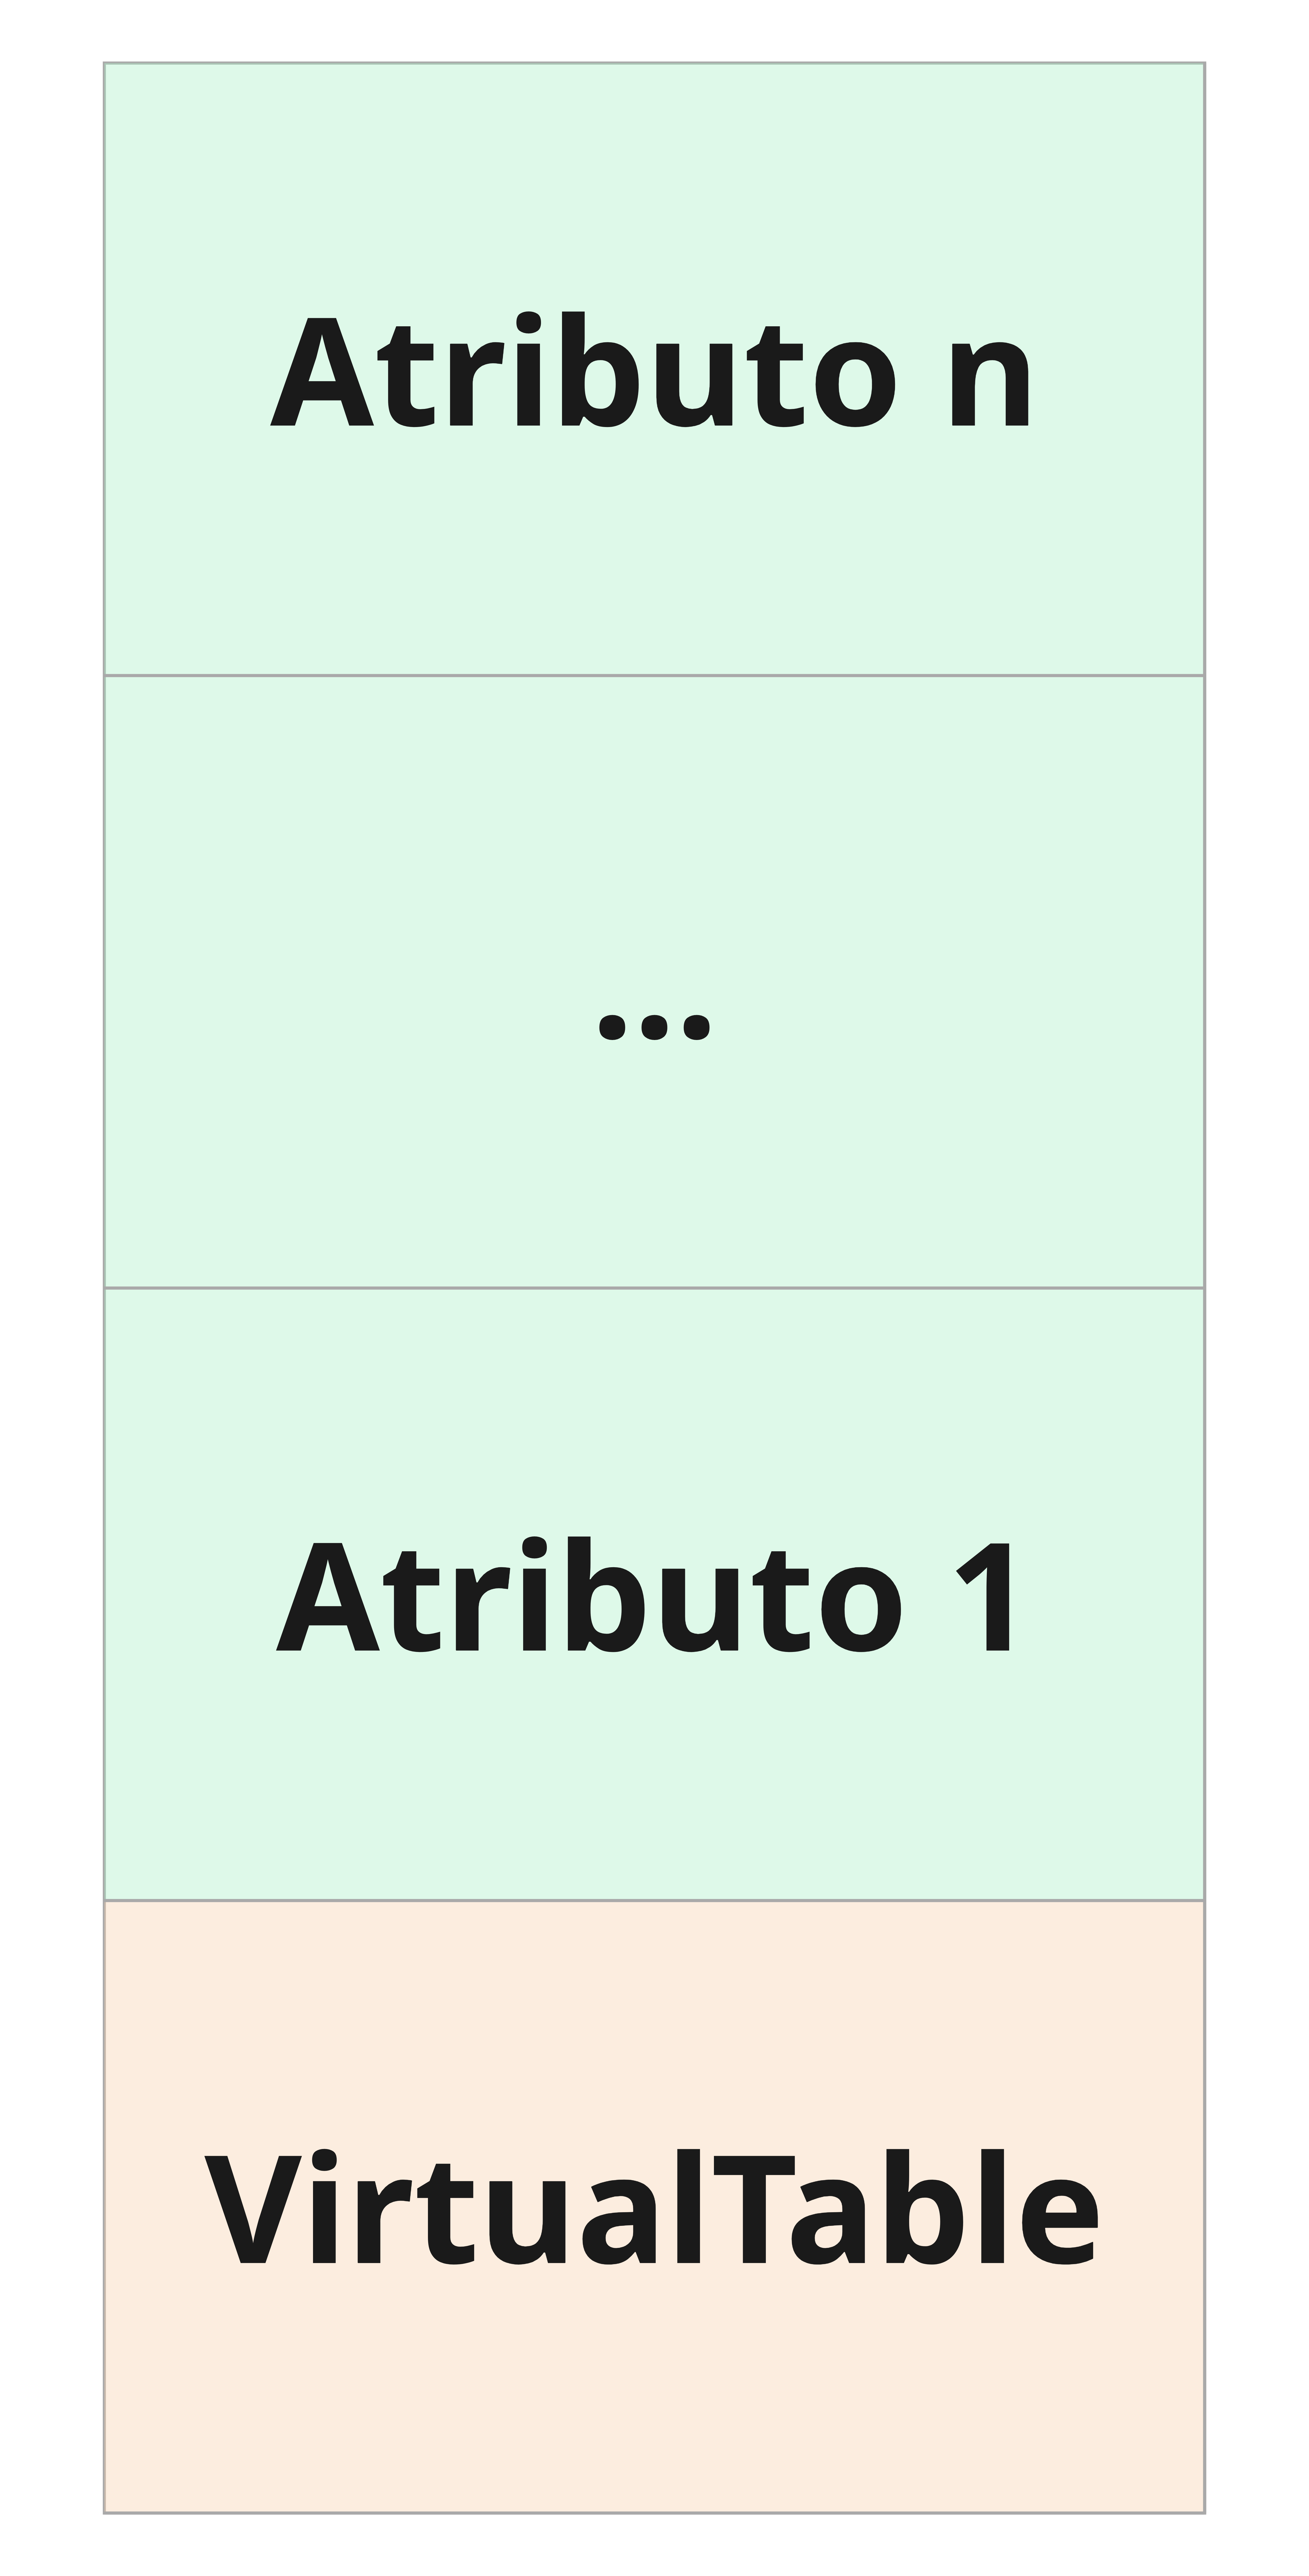
\includegraphics[width=0.3\linewidth]{img/CIR.png}
  \caption{Representación en memoria de un CIR}
  \label{fig:cir-valores-primitivos}
\end{figure}

\subsection{Objetos y atributos}
Una instancia se reserva en memoria dinámica. Su primera palabra apunta
a la virtual table de la clase, a continuación se almacenan los
atributos, según las posiciones que asignó la tabla de símbolos. El
desplazamiento de un atributo se calcula como
\lexcode{(position + 1) * 4}, porque la palabra inicial está ocupada por
la referencia a la virtual table.

La creación de una instancia prepara el objeto y ejecuta el constructor
correspondiente. La inicialización de atributos distingue los tipos
primitivos de los tipos de referencia: los primitivos reciben sus CIR
iniciales y las referencias a clases o arreglos parten de \texttt{nil}.
Luego se escribe en la primera palabra la tabla virtual de la clase
instanciada.

\subsection{Arreglos}
Un arreglo reserva una cabecera de dos palabras y, a continuación, una
palabra por elemento. La primera palabra de la cabecera referencia la
tabla virtual del tipo de arreglo y la segunda guarda su longitud. Cada
posición almacena la dirección del CIR de un elemento, la dirección del
elemento \texttt{i} se obtiene avanzando desde el desplazamiento de
cabecera y multiplicando el índice por cuatro.

Al crear un arreglo, el código reserva el espacio según su longitud e
inicializa cada posición con un CIR del tipo de elemento. Los accesos de
lectura y escritura comprueban que la referencia no sea nula y que el
índice se encuentre dentro de los límites. Las rutinas predefinidas de
iteración usan el estado del iterador para obtener los elementos.

\begin{figure}[H]
  \centering
  
\includegraphics[width=0.3\linewidth]{img/CIR_array.png}
  \caption{Representación en memoria de un arreglo y sus elementos.}
  \label{fig:cir-arreglo}
\end{figure}

\subsection{Cadenas}
Las cadenas literales se almacenan en \texttt{.data}. El generador
mantiene un mapa entre el lexema y su etiqueta para evitar volver a
emitir un literal ya registrado. La cadena vacía reutiliza la etiqueta
predefinida \texttt{empty\_str}. Los caracteres imprimibles se agrupan
en directivas \texttt{.ascii}, los escapes y bytes que no se representan
directamente se emiten con \texttt{.byte}. Cada cadena termina con un
byte nulo.

El analizador léxico admite los escapes de la tabla siguiente. Durante la
generación, \lexcode{CodeGenerator.emitStringContent()} convierte cada
escape en el byte indicado; los caracteres imprimibles consecutivos se
agrupan en una directiva \texttt{.ascii}.

\begin{center}
\small
\begin{tabular}{|c|l|r|}
\hline
\textbf{Escape} & \textbf{Carácter representado} & \textbf{Código decimal} \\ \hline
\texttt{\textbackslash n} & Salto de línea & 10 \\ \hline
\texttt{\textbackslash t} & Tabulación horizontal & 9 \\ \hline
\texttt{\textbackslash v} & Tabulación vertical & 11 \\ \hline
\texttt{\textbackslash r} & Retorno de carro & 13 \\ \hline
\texttt{\textbackslash "} & Comilla doble & 34 \\ \hline
\texttt{\textbackslash '} & Comilla simple & 39 \\ \hline
\texttt{\textbackslash\textbackslash} & Barra invertida & 92 \\ \hline
\end{tabular}
\end{center}

Los códigos numéricos son valores de byte decimales emitidos mediante
\texttt{.byte}. Por ejemplo, \texttt{\textbackslash n} se representa como
\texttt{.byte 10}, no como los dos caracteres \texttt{\textbackslash} y
\texttt{n}. Los caracteres ASCII imprimibles se escriben con
\texttt{.ascii}. El indicador de fin de texto \texttt{.byte 0}
se agrega una sola vez al final de cada cadena.

\section{Convención de llamadas y Registro de activación}
\label{sec:convencion-llamadas}

Los prólogos y epílogos se generan a partir de la cantidad y posición de
parámetros y variables locales de cada método. El registro de activación
usa \texttt{\$fp} como referencia dentro del registro: allí se guarda la dirección
de retorno; los parámetros, el resultado, el \texttt{self} y el
\texttt{\$fp} del llamador ocupan posiciones positivas, mientras que
las variables locales ocupan posiciones negativas.

\begin{figure}[H]
  \centering
  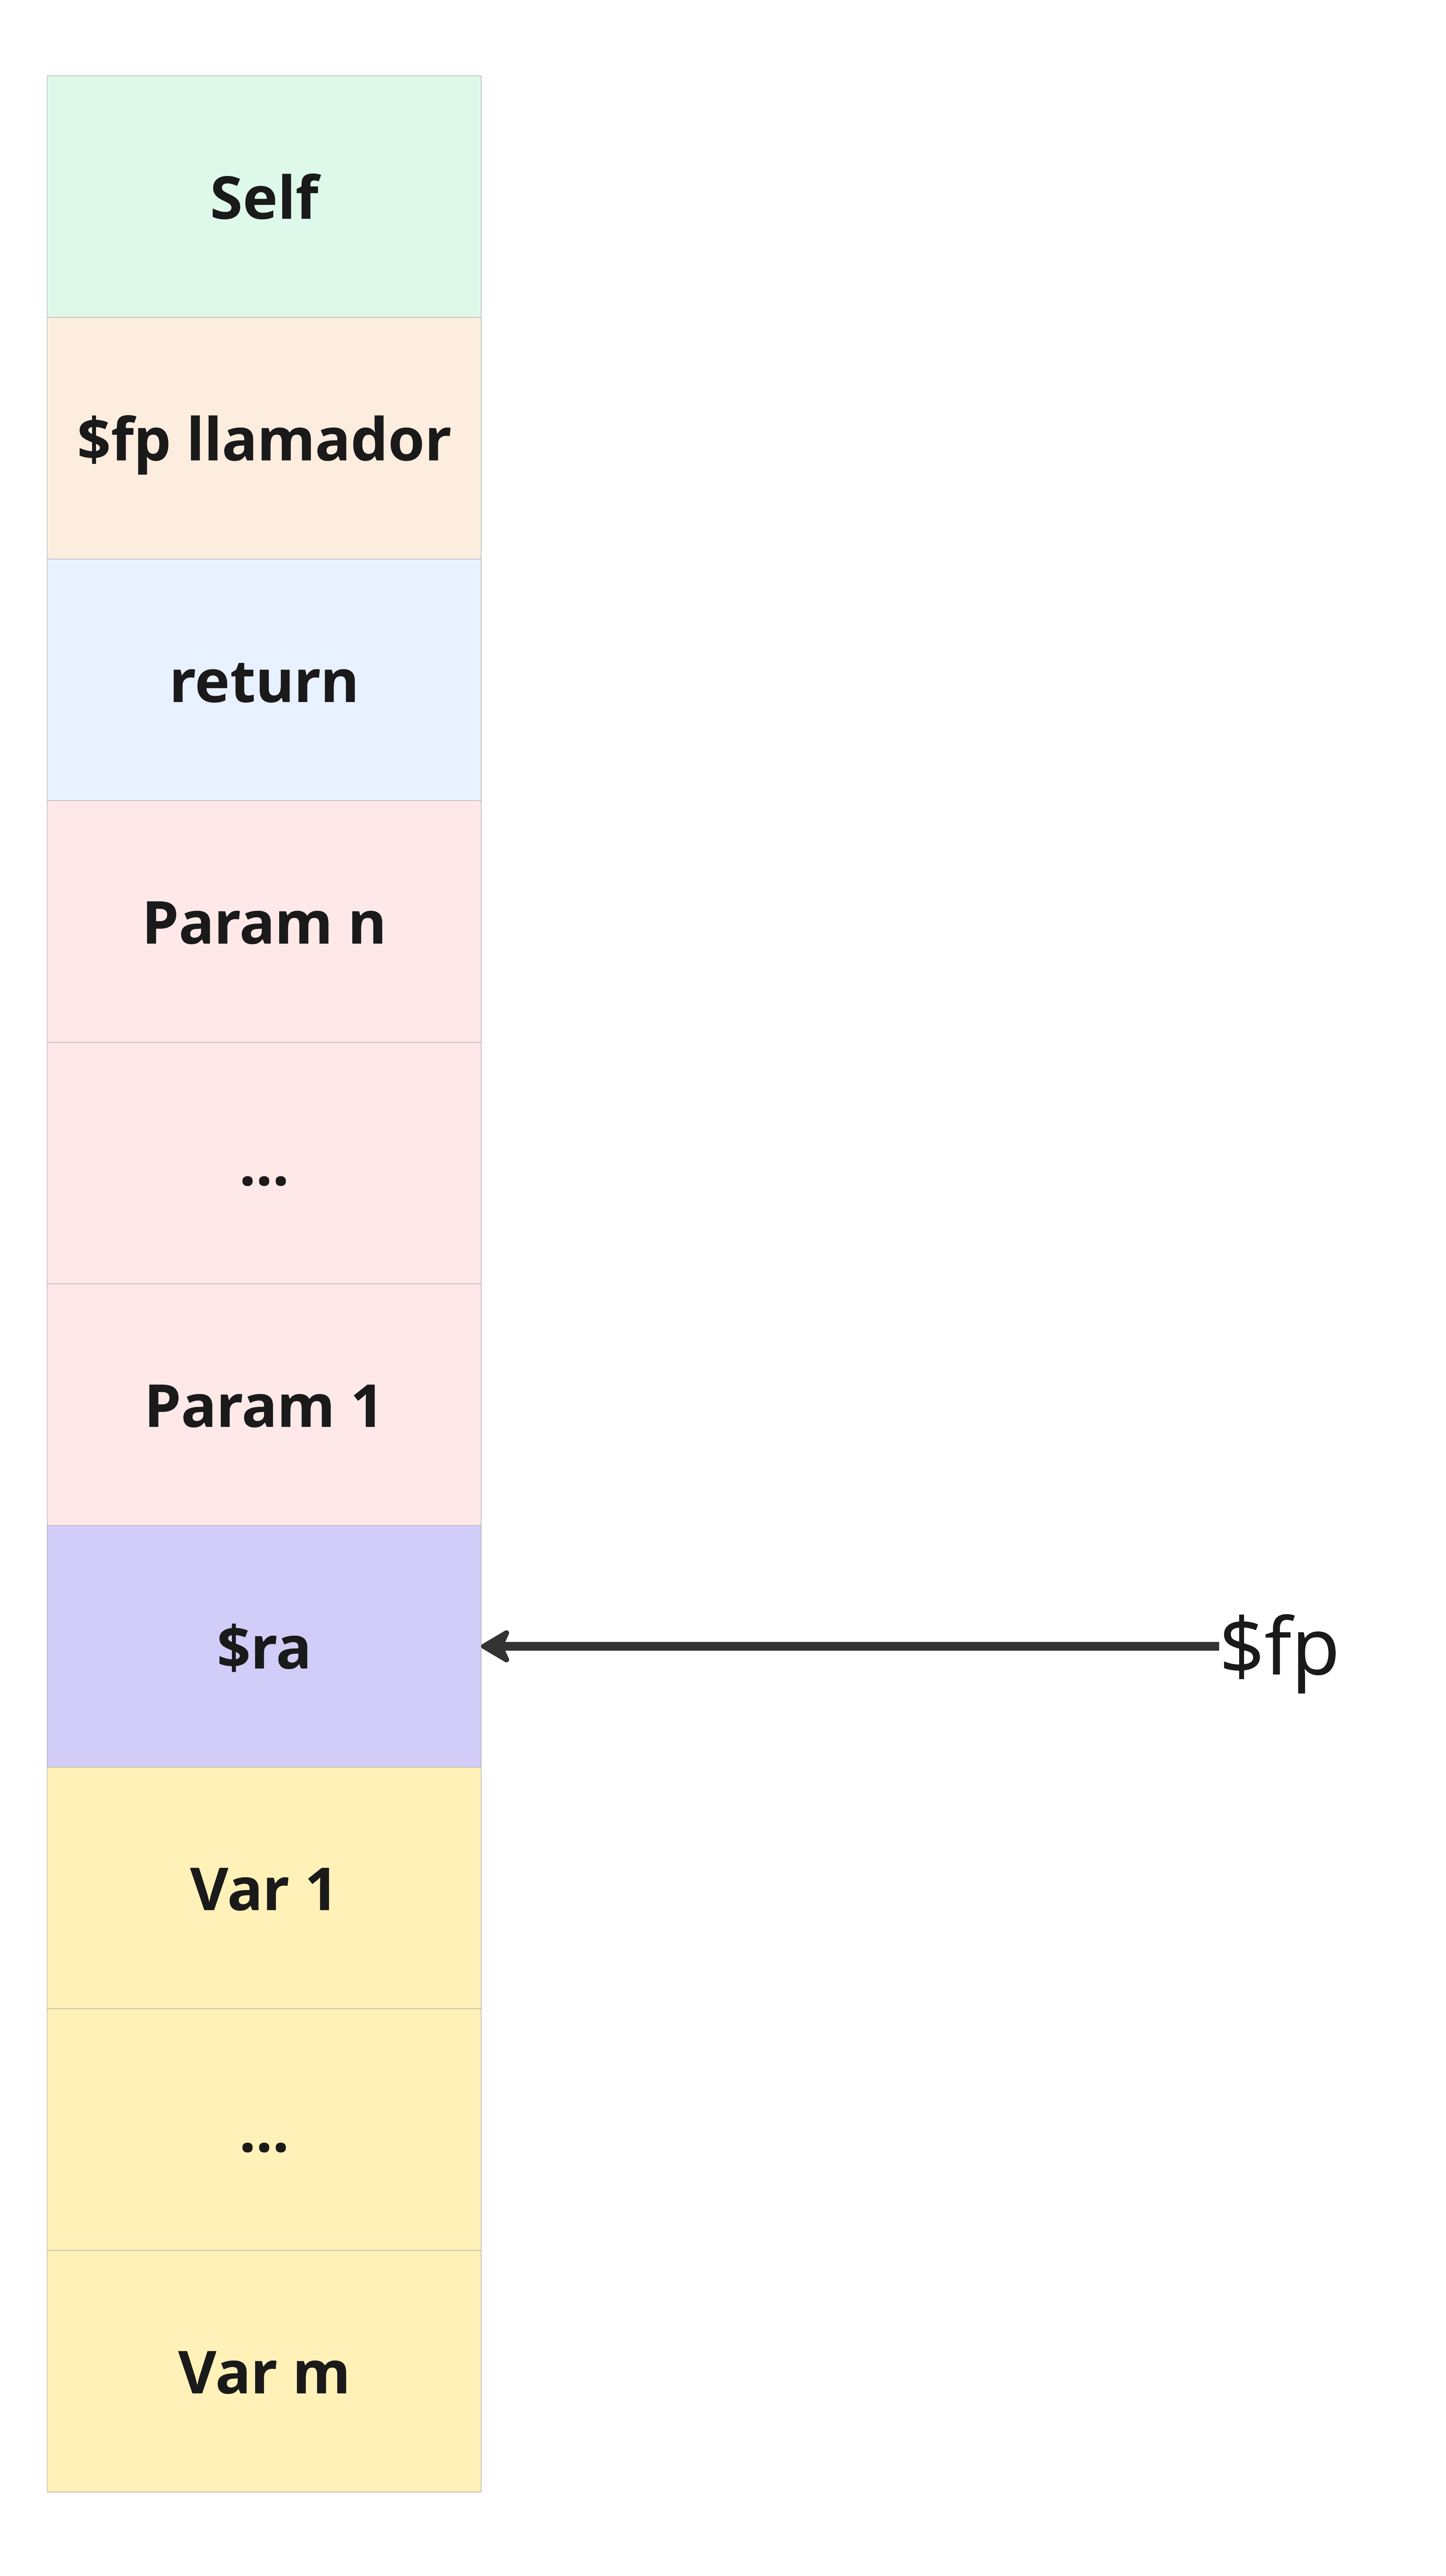
\includegraphics[width=0.4\linewidth]{img/registro_activacion.png}
  \caption{Representación de un registro de activación.}
  \label{fig:registro-activacion}
\end{figure}

Antes de una llamada, \lexcode{generateMethodPreCall()} reserva el área
correspondiente y guarda el contexto, el \texttt{\$fp} del llamador y el
espacio de retorno. El prólogo del método fija \texttt{\$fp}, guarda
\texttt{\$ra} y reserva el espacio para las variables locales. Al
finalizar, el epílogo recupera el resultado si existe, restaura el
contexto y retorna con \texttt{jr \$ra}. Los constructores retornan la
referencia de \texttt{self}; \texttt{start} finaliza el proceso mediante
el servicio de salida de MIPS.

\section{Estrategias de traducción}
\label{sec:estrategias-generacion}

\subsection{Expresiones}
Los literales generan su valor y, cuando son primitivos, construyen el
CIR correspondiente. En las expresiones binarias se evalúan los dos
operandos y se emiten instrucciones MIPS para suma, resta, multiplicación,
división, comparaciones y operaciones lógicas. Los operadores unarios
aplican la operación sobre el valor del operando. Las expresiones
parentizadas delegan en la expresión contenida.

Las llamadas preparan el contexto de activación, evalúan los argumentos
y transfieren el control al método o rutina predefinida. El resultado,
cuando corresponde, se recupera desde el espacio de retorno. Los
accesos encadenados actualizan el receptor durante el recorrido. En las
llamadas de instancia, la resolución dinámica utiliza la tabla virtual
del objeto; los métodos estáticos se llaman según su etiqueta.

\subsection{Asignaciones y accesos}
El lado izquierdo de una asignación determina la ubicación que recibirá
el resultado: puede ser una variable local, un parámetro, un atributo o
un elemento de arreglo. El lado derecho se evalúa y su referencia o valor
se almacena en la ubicación resuelta. Los accesos a atributos usan el
desplazamiento calculado a partir de la posición del atributo. Para
acceder a un arreglo se calcula primero la dirección del elemento,
después de validar la referencia y el índice.

\subsection{Sentencias de control}
Las sentencias condicionales y los ciclos se traducen con etiquetas y
saltos. Una condición falsa dirige el flujo a la etiqueta que corresponde
a la rama alternativa o a la salida del ciclo. Los cuerpos anidados
generan sus propias etiquetas. El contador \lexcode{forDepth} del
generador permite mantener el nivel de anidamiento de los recorridos.
Las sentencias de retorno escriben el resultado en el registro actual y
transfieren la ejecución al epílogo del método.

\subsection{Entrada y salida}
Las operaciones de entrada y salida utilizan rutinas incluidas en
\lexcode{text.asm}. El entorno contempla lectura de enteros, cadenas y
booleanos; impresión de esos tipos y de arreglos; y operaciones de
cadenas y arreglos como longitud, concatenación e iteración. Los
argumentos y resultados de estas rutinas respetan la misma convención de
registros de activación que los métodos generados.

\section{Controles durante la ejecución}
\label{sec:controles-runtime}

Algunos errores no se pueden detectar solo con el análisis estático,
porque dependen del valor concreto que se produzca durante la
ejecución. El código generado incorpora saltos a rutinas de error para
los casos siguientes:

\begin{description}[style=nextline]
  \item[División por cero]
  Antes de dividir, se comprueba si el divisor es cero. En ese caso se
  transfiere el control a \texttt{runtime\_div\_zero}.
  \item[Referencia nula]
  Antes de acceder a miembros o elementos de una referencia, se valida
  que no sea cero. \texttt{runtime\_null} informa la línea y la columna
  asociadas al acceso.
  \item[Índice negativo]
  La comprobación del índice transfiere el control a
  \texttt{runtime\_negative\_index} si el valor es menor que cero.
  \item[Índice fuera de rango]
  Se compara el índice con la longitud del arreglo. Un índice igual o
  mayor que la longitud conduce a \texttt{runtime\_out\_of\_range}.
\end{description}

Las rutinas imprimen el mensaje definido en \lexcode{data.asm} y
finalizan el programa. Estos casos no son errores de generación: el
compilador produce el ensamblador y la condición se informa al ejecutar
el programa resultante.

\section{Formato del ensamblador generado}
\label{sec:formato-asm}

El archivo final contiene las secciones estándar \texttt{.data} y
\texttt{.text}. En datos aparecen las cadenas predefinidas, las
etiquetas de los literales del programa y las tablas virtuales. En texto
se declara \texttt{main} como símbolo global, se genera el bloque
\texttt{start}, se incorporan las rutinas del entorno y se agregan los
métodos y constructores del programa.

El generador incluye comentarios en el ensamblador para identificar
prólogos, epílogos, bloques de código, expresiones y controles. Estos
comentarios facilitan relacionar instrucciones con el nodo o la
operación TinyS que las originó. Las etiquetas de control se construyen
para distinguir los distintos puntos de salto generados.


\section{Errores de compilación}
\label{sec:errores-generacion}

La generación ocurre únicamente después de que el programa supera las
etapas léxica, sintáctica y semántica. Si alguna etapa falla, el
ejecutador informa el encabezado de la fase y su diagnóstico, y no
escribe nuevas salidas para esa ejecución. Si se produce una excepción
semántica durante el armado del AST, también se informa bajo la fase
semántica correspondiente. Una compilación exitosa guarda los resultados
JSON y el archivo ensamblador con el nombre base del fuente.

\section{Escenarios y casos de prueba}
\label{sec:casos-generacion}

Las pruebas de generación están implementadas en
\lexcode{CodeGenTest}. El conjunto recorre los programas de
\lexcode{tc/tinyS/success} y
\lexcode{tc/tinyS/error}; para cada fuente ejecuta el
analizador y escribe el ensamblador en
\lexcode{tc/tinyS/mipsFiles}.

\subsection{Casos que deben generarse}
Los ejemplos de \texttt{success} cubren literales y expresiones,
operaciones aritméticas y relacionales, entrada y salida, cadenas,
arreglos, constructores, llamadas con argumentos, métodos estáticos y
de instancia, herencia, condicionales, ciclos y retornos en ramas. Las
salidas \texttt{.asm} permiten inspeccionar el código que produce cada
caso.

\subsection{Casos con error en tiempo de ejecución}
Los ejemplos de \texttt{error} también deben superar la compilación y
generar ensamblador. Comprueban que se emitan las verificaciones para
división por cero, referencias nulas e índices negativos o fuera del
rango. La clase de pruebas aclara que el error se produce al ejecutar
el MIPS, por lo que estos casos no deben confundirse con fuentes que el
compilador rechaza.

\endgroup
